\documentclass[12pt, a4paper]{article}

\usepackage{ctex} % 使用ctex宏包支持中文
\usepackage{geometry} % 页面设置
\usepackage{amsmath, amssymb, ntheorem} % 数学公式
\usepackage{graphicx} % 插入图片
\usepackage{enumitem} % 列表环境
\usepackage{hyperref} % 超链接
\usepackage{tikz}
\usepackage{tikz-qtree}

% 页面设置
\geometry{left=2.5cm, right=2.5cm, top=2.5cm, bottom=2.5cm}

% 标题信息
\title{课后练习4}
\author{}
\date{}

\begin{document}

\maketitle % 显示标题

\section{问题一}

\subsection{}

设四个属性分别为$O,T,H,W$,则我们可以分别计算它们对应的information gain.

\begin{align*}
    H(D)&=-(\frac{9}{14}\log\frac{9}{14}+\frac{5}{14}\log\frac{5}{14})\approx0.94029\\
    g(D,O)&=H(D)-H(D\vert O)\\
    &=H(D)-\bigl(\frac{5}{14}[-(\frac{3}{5}\log\frac{3}{5}+\frac{2}{5}\log\frac{2}{5})]
    +\frac{4}{14}[-(\frac{4}{4}\log\frac{4}{4})]
    +\frac{5}{14}[-(\frac{3}{5}\log\frac{3}{5}+\frac{2}{5}\log\frac{2}{5})]\bigr)\\
    &=0.24675\\
    g(D,T)&=H(D)-H(D\vert T)\\
    &=H(D)-\bigl(\frac{4}{14}[-(\frac{2}{4}\log\frac{2}{4}+\frac{2}{4}\log\frac{2}{4})]
    +\frac{6}{14}[-(\frac{4}{6}\log\frac{4}{6}+\frac{2}{6}\log\frac{2}{6})]
    +\frac{4}{14}[-(\frac{1}{4}\log\frac{1}{4}+\frac{3}{4}\log\frac{3}{4})]\bigr)\\
    &=0.029227\\
    g(D,H)&=H(D)-H(D\vert H)\\
    &=H(D)-\bigl(\frac{7}{14}[-(\frac{3}{7}\log\frac{3}{7}+\frac{4}{7}\log\frac{4}{7})]
    +\frac{7}{14}[-(\frac{1}{7}\log\frac{1}{7}+\frac{6}{7}\log\frac{6}{7})]\bigr)\\
    &=0.15184\\
    g(D,W)&=H(D)-H(D\vert W)\\
    &=H(D)-\bigl(\frac{8}{14}[-(\frac{2}{8}\log\frac{2}{8}+\frac{6}{8}\log\frac{6}{8})]
    +\frac{6}{14}[-(\frac{3}{6}\log\frac{3}{6}+\frac{3}{6}\log\frac{3}{6})]\bigr)\\
    &=0.04813\\
\end{align*}

根据计算得到的information gain,我们可以相应建树:

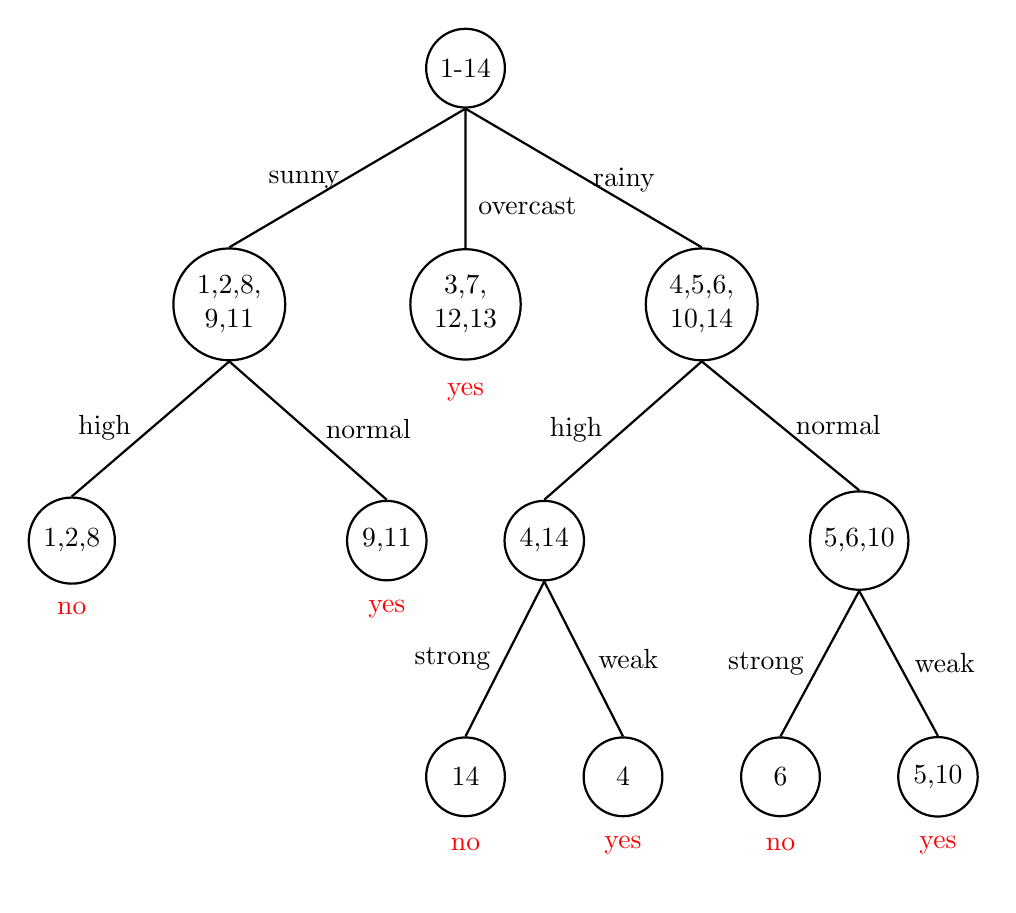
\begin{tikzpicture}[transform shape, thick,
    every node/.style = {draw, circle, minimum size = 10mm},
    grow = down,
    level 1/.style={sibling distance=3cm},
    level 2/.style={sibling distance=4cm},
    level 3/.style={sibling distance=2cm},
    level distance=3cm]
\node (A){1-14}
    child {node[align=center] (B){1,2,8,\\9,11}
        child {node (E){1,2,8}}
        child {node (F){9,11}}}
    child {node[align=center] (C){3,7,\\12,13}}
    child {node[align=center] (D){4,5,6,\\10,14}
        child {node (G){4,14}
            child {node (I){14}}
            child {node (J){4}}}
        child {node (H){5,6,10}
            child {node (K){6}}
            child {node (L){5,10}}}};
            

\begin{scope}[nodes = {draw = none}]
    \path (A)     -- (B) node [midway, left]  {sunny};
    \path (A)     -- (C) node [pos=0.7, right] {overcast};
    \path (A)     -- (D) node [midway, right] {rainy};
    \path (B)     -- (E) node [midway, left] {high};
    \path (B)     -- (F) node [midway, right] {normal};
    \path (D)     -- (G) node [midway, left] {high};
    \path (D)     -- (H) node [midway, right] {normal};
    \path (G)     -- (I) node [midway, left] {strong};
    \path (G)     -- (J) node [midway, right] {weak};
    \path (H)     -- (K) node [midway, left] {strong};
    \path (H)     -- (L) node [midway, right] {weak};
    \begin{scope}[nodes = {below = 17pt, text = red}]
        \node at (C) {yes};
    \end{scope}
    \begin{scope}[nodes = {below = 10pt, text = red}]
        \node at (E) {no};
        \node at (F) {yes};
        \node at (I) {no};
        \node at (J) {yes};
        \node at (K) {no};
        \node at (L) {yes};
    \end{scope}
\end{scope}


\end{tikzpicture}

\subsection{}

根据得到的树模型可知,此时到达了\{9,11\}节点,应该进行户外活动

\section{问题二}

\subsection{}

使用Bootstrapping方法,从$N$个样本中每次选一个,有放回地选择$N'=pN$次,那么一个样本未被选中的概率即为
\begin{align*}
    P &= (1-\frac{1}{N})^{N'}\\
    &=(1-\frac{1}{N})^{pN}
\end{align*}
当N趋于无穷时,
\begin{align*}
    &\lim_{N \to \infty}(1-\frac{1}{N})^{pN}\\
    =&\bigl(\lim_{N \to\infty}(1-\frac{1}{N})^N\bigr)^p\\
    =&(\frac{1}{e})^p\\
    =&e^{-p}
\end{align*}
因此总共有$N\cdot e^{(-p)}$个样本不会被采样到

\subsection{}

一个样本被分类错误,当且仅当有至少两个决策树的分类是错误的. 因此被错误分类的总概率为
\begin{align*}
    E(G)&=E(g_1)E(g_2)E(g_3)+E(g_1)E(g_2)(1-E(g_3))+E(g_1)(1-E(g_2))E(g_3)+(1-E(g_1))E(g_2)E(g_3)\\
    &=0.15\times0.25\times0.3+0.15\times0.25\times0.7+0.15\times0.75\times0.3+0.85\times0.25\times0.3\\
    &=0.135
\end{align*}

\section{问题三}

\subsection{}

已知平方损失函数为
\begin{align*}
    L(h)=\sum_{(x_i,y_i)\in D}(y_i-g^{(T)}(x_i))^2
\end{align*}
设第$t$步得到的$g^{(t)}(x_i)$与$y_i$的残差为$r_i^{(t)}$:
\begin{align*}
    r_i^{(t)}=y_i-g^{(t)}(x_i)
\end{align*}
求偏导得到
\begin{align*}
    \frac{\partial L}{\partial \alpha_t}&=\sum_{(x_i,y_i)\in D}2(y_i-g^{(T-1)}(x_i)-\alpha_t f_t(x_i))(-f_t(x_i))=0\\
    &\Leftrightarrow\sum_{(x_i,y_i)\in D}(y_i-g^{(T-1)}(x_i)-\alpha_t f_t(x_i))f_t(x_i)=0\\
    &\Leftrightarrow\sum_{(x_i,y_i)\in D}f_t(x_i)(y_i-g^{(T-1)}(x_i))=\alpha_t \sum_{(x_i,y_i)\in D}f_t^2(x_i)
    \quad (f_t^2(x_i)=1)\\
    &\Leftrightarrow\quad\alpha_t = \frac{\sum_{(x_i,y_i)\in D}f_t(x_i)r_i^{T-1}}{\vert D \vert}
\end{align*}

\subsection{}

$T$最小为2,如图所示,对于$f_1$,有两个点被分错,于是
\begin{align*}
    e_1&=0.4\\
    \alpha_1&=\frac{1}{2}\log(1.5)=0.2027
\end{align*}
可以更新参数得到
\begin{align*}
    &\bar{w}_1^{(2)}=\bar{w}^{(2)}_2=0.2449\\
    &\bar{w}^{(2)}_3=\bar{w}_4^{(2)}=\bar{w}_5^{(2)}=0.1633\\
    &w_1^{(2)}=w_2^{(2)}=0.245\\
    &w_3^{(2)}=w_4^{(2)}=w_5^{(2)}=0.167
\end{align*}
对于$f_2$,同样有两个点被分错
\begin{align*}
    e_2&=0.334\\
    \alpha_2&=\frac{1}{2}\log(0.666/0.334)=0.151
\end{align*}
可以发现此时$f_1$和$f_2$就可以将数据集正确分类,因此$T_{min}=2$

\begin{figure*}
    \centering
    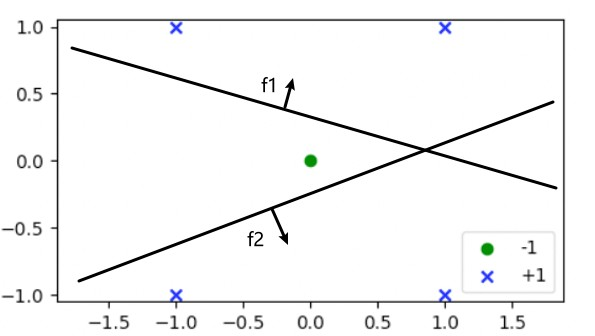
\includegraphics{img/a4_1.jpg}
\end{figure*}

\subsection{}

可以从以下几个角度来缓解Adaboost过拟合:
\begin{enumerate}
    \item 增大数据集
    \item 降低弱分类器$f_t$的复杂度
    \item 增加正则化项,使用L1或L2正则化
\end{enumerate}

\section{问题四}

\subsection{}



\subsection{}



\subsection{}



\end{document}
